
\chapter{O Problema de Sintonia} \label{chap:conc}
	

A sintonia de simuladores de poços de petróleo costuma ser feita a partir de dados experimentais. 
%
A partir de testes de campo, adquirem-se pontos de testes do sistema real.
%
Os pontos reais são utilizados como referência para que o operador varie os parâmetros de forma a encontrar o modelo que melhor represente os dados coletados.
%

Para os testes neste trabalho, primeiramente foi configurado um único poço de petróleo, com uma estrutura simples e que pode ser visto na figura \ref{fig:setup1_dia}.
% 
A seguir foram escolhidos dados arbitrariamente para compor a curva ``real'' de produção (figura \ref{fig:truth1}).
%
Neste Experimento a curva sintonizada foi a de fluxo de líquido (Barris padrões por dia) por gás injetado (milhões de pés cúbicos padrões por dia), no entanto é possível utilizar outras curvas, ou ainda mais que uma, para a sintonia.
%

Escolheu-se a pressão estática do reservatório como sendo 4000 psi absoluto, e um índice de produtividade de líquido de 25 STDB/d/psi (barris padrões por dia por pressão estática). 
%
Desta forma a figura \ref{fig:truth1} demonstra o poço ``real'' a ser sintonizado.



\begin{figure}[H]
\centering
\begin{subfigure}{.25\textwidth}
  \centering
  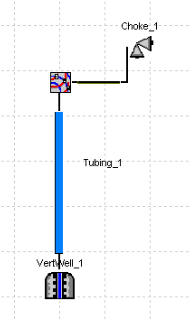
\includegraphics[width=1\linewidth]{figs/setup1.png}
  \caption{Setup do poço de petróleo.}
  \label{fig:setup1_dia}
\end{subfigure}%
\begin{subfigure}{.75\textwidth}
  \centering
  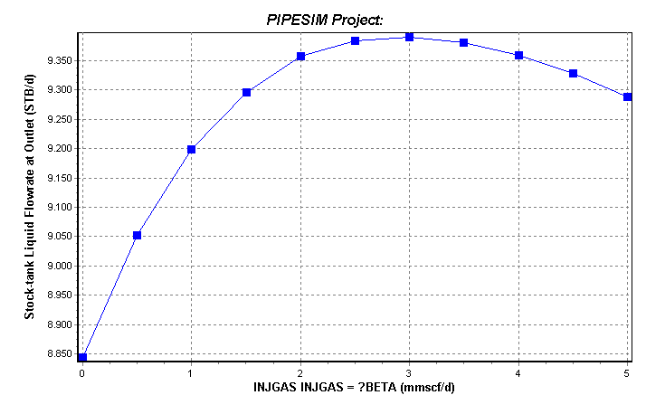
\includegraphics[width=1\linewidth]{figs/truth1.png}
  \caption{Curva ``real'' do poço de petróleo.}
  \label{fig:truth1}
\end{subfigure}
\caption{Configuração e curva do poço do experimento 1.}
\label{fig:setup1}
\end{figure}

Em todos os testes, os parâmetros $s_p$ (pressão estática) e $l_{pi}$ (Índice de produção de líquido) foram iniciados respectivamente em 3000 (psi) e 15 (STDB/d). A interface OpenLink foi utilizada para modificar os parâmetros e ler uma nova curva de fluxo de líquido por injeção de gás, a distância quadrática entre as duas curvas foi utilizada como o erro na otimização.

O problema de otimização, então, é dado por 
\begin{align}
\min\limits_{x \in \Omega} f(x)
\end{align}
Aonde
\begin{align}
x = &(s_p, l_{pi})\\
\Omega = &\{s_p \in \mathbb{R} \mid s_{p,min} < s_p < s_{p,max}\}\\
          &\{l_{pi} \in \mathbb{R} \mid  l_{pi,min} < l_{pi} < l_{pi,max}\}
\end{align}
Aonde $s_p$ é a pressão estática do reservatório e $l_{pi}$ é o índice de produtividade de líquidos, e seja $f(q_{inj};x)$ a produção de líquido estimada pelo simulador quando sintonizado com parâmetros $x$. 

Seja $\theta(q_{inj};x)$ a produção ``real'' de líquido com parâmetros $x$.
\begin{align}
f(x) &= f(s_p, l_{pi}) \\
     &= \sum_{i=1}^n \Big[ \theta(q_{inj}^n;x) - f(q_{inj}^n;x))\Big]^2
\end{align}
Onde $q_{inj}^1, q_{inj}^2, \dots, q_{inj}^n$ são os pontos amostrados da curva de produção. 

Neste problemas foram impostos: 
\begin{align*}
l_{pi,min}&= 15\\
l_{pi,max}&= 35\\
s_{p,min} &= 2000\\
s_{p,max} &= 7000\\
\end{align*}
\chapter{O Experimento de Sintonia Sem Ruído}

Foram realizados três experimentos de sintonia de curva, e utilizadas três abordagens diferentes para a sintonia. Primeiramente foi utilizado o orthoMADS, com a implementação NOMAD, em seguida, foi utilizado novamente o NOMAD, mas com um surrogate model calculado pela SGTELIB, e finalmente, uma implementação do Nelder-Mead Simplex. Os resultados então são comparados quanto a número de avaliações e acurácia do resultado.

Os experimentos foram realizados em uma máquina virtual VirtualBox, rodando em um Xeon 2665, e utilizando dois núcleos.

\section{Setup para sintonia de curva com o orthoMADS}
Para a sintonia com o orthoMADS, foi utilizado o framework OPAL (A Framework for Optimization of Algorithms), interface Python para o solver NOMAD.
A implementação com o OPAL utiliza dois arquivos, "well\_declaration.py" e "well\_optimize.py".

O arquivo "well\_declaration.py" expõe os componentes do problema:

\begin{itemize}
\item Nome do algoritmo:
\begin{lstlisting}[language=Python]
# Define Algorithm object.
tuning = Algorithm(name='TUNING', description='Well Tuning')
\end{lstlisting}
\end{itemize}

\begin{itemize}
\item Comando utilizado pelo solver para avaliar a função:
\begin{lstlisting}[language=Python]
tuning.set_executable_command('python pipesim_run.py')
\end{lstlisting}
\end{itemize}


\begin{itemize}
\item As variáveis de decisão:
\begin{lstlisting}[language=Python]
static_pressure = Parameter(kind='real', 
                            default=sp, 
                            bound=(2000, 7000),
                            name='sp', 
                            description='Static Pressure')
liq_pi = Parameter(kind='real', 
                   default=pi, 
                   bound=(15, 35),
                   name='pi', 
                   description='Liq PI')

FD.add_param(static_pressure)
FD.add_param(liq_pi)
\end{lstlisting}
\end{itemize}

\begin{itemize}
\item E o erro:
\begin{lstlisting}[language=Python]
error = Measure(kind='real', name='ERROR', description='Curve quadratic error')
FD.add_measure(error)
\end{lstlisting}
\end{itemize}

Já no arquivo "well\_optimize", são declaradas estruturas auxiliares:
\begin{itemize}

\item É instanciado o solver:
\begin{lstlisting}[language=Python]%

def get_error(parameters, measures):
    return sum(measures["ERROR"])

data = ModelData(FD)
struct = ModelStructure(objective=get_error)  # Unconstrained
model = Model(modelData=data, modelStructure=struct)

NOMAD = NOMADSolver()

\end{lstlisting}



\item São impostas as seguintes restrições ao solver do NOMAD:
\begin{lstlisting}[language=Python]
F_TARGET = 0.1
\end{lstlisting}

De modo a limitar o tamanho mínimo da malha, e terminar a simulação quando a função custo chegar a um valor abaixo de 0.1

\item E é inicilizada a otimização:
\begin{lstlisting}[language=Python]
NOMAD.solve(blackbox=model)
\end{lstlisting}

\end{itemize}

\section{Resultados da Sintonia de Curva com o orthoMADS}

Em 525 segundos (8:45 minutos) e com de 206 avaliações de caixa preta. A performance do algoritmo pode ser vista na figura \ref{fig:setup1_2}. A parada se deu pelo valor da função custo estar abaixo de 0,1. A convergência se deu para os seguintes valores:

\begin{align*}
s_p&= 4000,691 \\
l_{pi} &= 24,954 \\
Custo &= 0,0757.
\end{align*}

Que são muito próximos aos valores reais $s_p=4000$ e $l_{pi}=25$.


\begin{figure}[H]
\centering
\begin{subfigure}{0.5\textwidth}
  \centering
  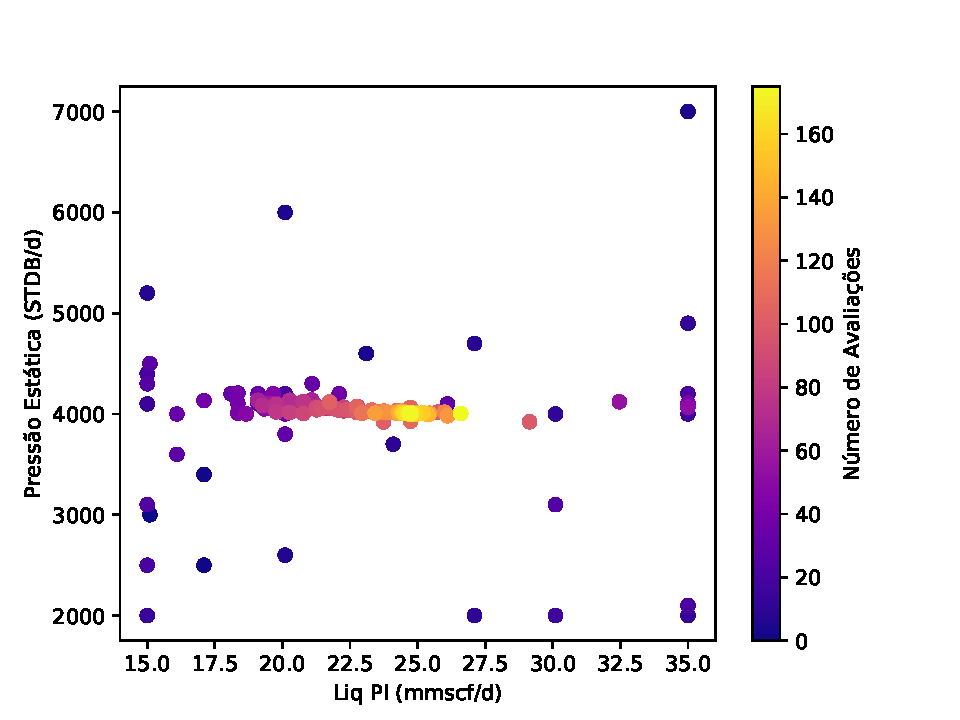
\includegraphics[width=1\linewidth]{figs/setup1_eval_points.pdf}
  \caption{Pontos escolhidos pelo NOMAD.}
  \label{fig:setup1_points}
\end{subfigure}%
\begin{subfigure}{0.5\textwidth}
  \centering
  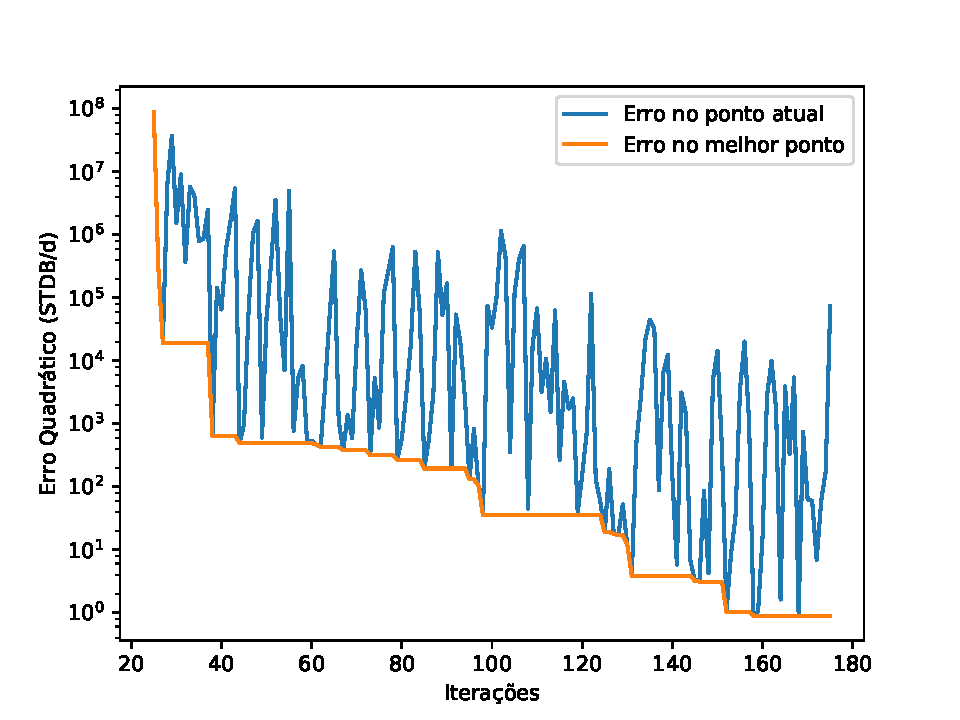
\includegraphics[width=1\linewidth]{figs/setup1_errors.pdf}
  \caption{Erro nos pontos avaliados.}
  \label{fig:setup1_error}
\end{subfigure}
\caption{NOMAD aplicado ao experimento 1.}
\label{fig:setup1_2}
\end{figure}

\section{A Surrogate Lib}

Durante a realização desses experimentos, o NOMAD foi atualizado e recebeu uma ferramenta auxiliar, uma biblioteca que tenta aproximar a função a partir dos pontos já utilizados, para utilização no passo "search" do algoritmo. Esta biblioteca faz com que o algoritmo, a cada iteração, tente adivinhar a melhor direção para avançar, ao invés de progredir aleatoriamente.

Para o cálculo do modelo substituto, são possíveis nove tipos de modelos, que podem ser vistos na documentação, além de onze tipos possíveis de núcleos. Neste trabalho foram utilizadas as opções padrão do NOMAD, um modelo PRS (Polynomial Response Surface) de ordem 2.


\section{Setup Para Sintonia de Curva Com a Surrogate Lib}

Um contra-tempo quanto a SGTELIB, como é chamada a biblioteca, é que ela está embutida nos binários do NOMAD, e, por algum erro, os binários para windows foram compilados com uma versão antiga do Microsoft Visual Studio, de forma que é necessário recompilar não apenas o SGTELIB (o que pode ser feito com o mingW sem grandes mudanças), mas todo o NOMAD, necessitando a instalação de aproximadamente 4Gb do Visual Studio.

Após sua recompilação, bastou substituir o binário antigo pelo novo, é inserir nos parâmetros do NOMAD para o uso da SGTELIB, com seus valores padrõess:
\begin{lstlisting}[language=Python]
NOMAD.set_parameter(name="MODEL_SEARCH", value="SGTELIB")
\end{lstlisting}
Para que ele passasse a utilizar o SGTELIB no local do seu SEARCH baseado em modelo quadrático.


\section{Resultados da Otimização Com a Surrogate Lib}

A execução demorou 1374 segundos (22:27 minutos) e necessitou de 417 avaliações de função de caixa preta. O Nomad novamente convergiu, desta vez para os 	valores:

\begin{align*}
s_p&= 4001,389 \\
L_{pi} &= 24,905 \\
Custo &= 0,09986.
\end{align*}
É possível notar, no entanto, que com o SGTELIB, em muitos pontos o erro quadrático saturou em $10^{64}$. Nota-se também que pontos longe do ótimo foram avaliados perto da convergência (pontos claros no canto inferior esquerdo), o que pode significar que existe um problema com a SGTELIB, ou que o modelo utilizado não é o ideal, talvez pelo fato de que as superfícies polinomiais tendam a crescer muito para longe na origem, levando o algoritmo a testar pontos distantes.

\begin{figure}
\centering
\begin{subfigure}{0.5\textwidth}
  \centering
  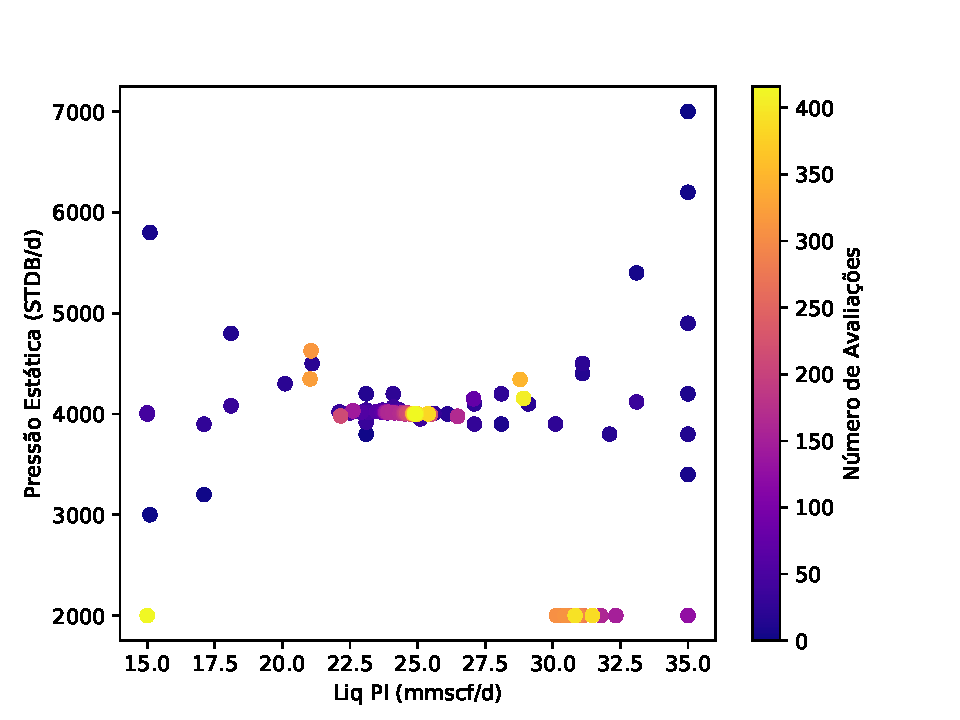
\includegraphics[width=1\linewidth]{figs/setup1sgtelib_eval_points.pdf}
  \caption{Pontos escolhidos pelo NOMAD.}
  \label{fig:setup2_points}
\end{subfigure}%
\begin{subfigure}{0.5\textwidth}
  \centering
  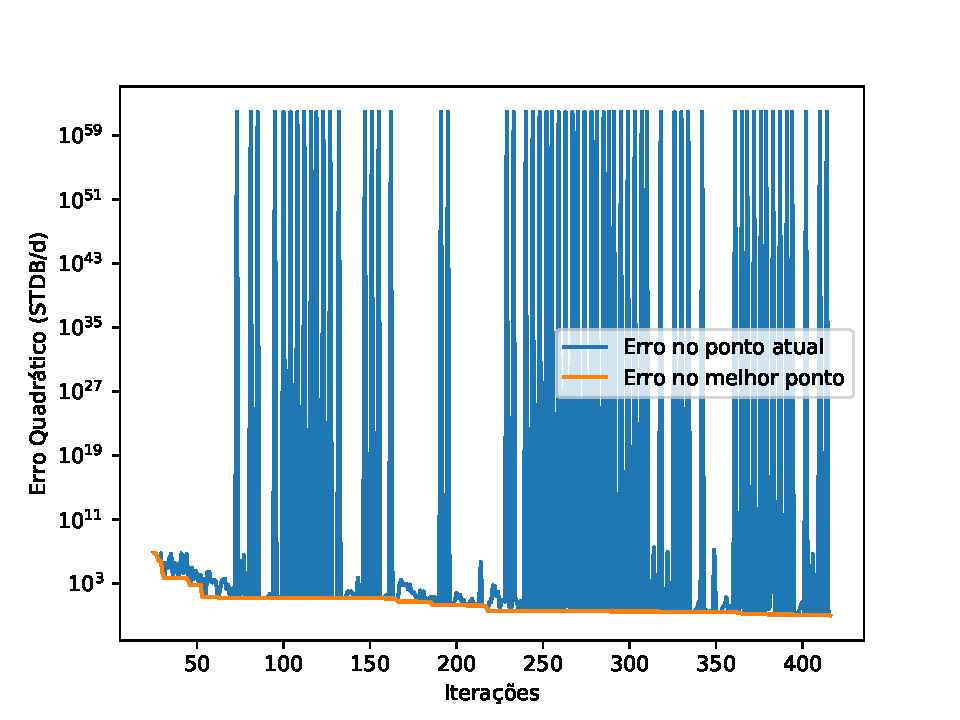
\includegraphics[width=1\linewidth]{figs/setup1sgtelib_errors.pdf}
  \caption{Erro nos pontos avaliados.}
  \label{fig:setup2_error}
\end{subfigure}
\caption{NOMAD aplicado ao experimento 1 com SGTELIB.}
\label{fig:setup2_2}
\end{figure}


\section{Setup da Otimização com Nelder-Mead Simplex}

Para o teste com o Simplex de Nelder-Mead, foi utilizada uma implementação própria, baseada no algoritmo \ref{alg:nm}, e como ele não é facilmente paralelizável, não houveram preocupações com paralelismo.
Os limites utilizados foram os mesmos dos casos anteriores:
\begin{align}
15 < &l_{pi} < 35 \\
2000 < &s_p < 7000
\end{align}

Como o simplex utiliza uma estrutura $n$-dimensional para a busca, são necessários $n+1$ pontos iniciais, por este motivo um triângulo foi expandido arbitrariamente a partir do ponto inicial, de modo que no começo do algoritmo, o simplex inicial seja grande. As restrições foram aplicadas somando-se um peso adicional a função custo.

Os resultados podem ser vistos nas figuras \ref{fig:setup3_2} e \ref{fig:setup3_triang}. Nota-se que a solução foi mais rápida, com 212 iterações em 133 segundos (2:13 minutos). No entanto, o método de Nelder e Mead não tem as mesmas características de convergência que os os métodos MADS. É interessante comentar o caso da figura 5, aonde é possível notar que o simplex primeiramente moveu-se para um ponto em torno de $l_{pi}=18$, depois moveu-se lentamente para o ponto final:

\begin{align*}
s_p&= 4001,389 \\
l_{pi} &= 24,905 \\
Custo &= 0,09986.
\end{align*}


\begin{figure}
\centering
\begin{subfigure}{0.5\textwidth}
  \centering
  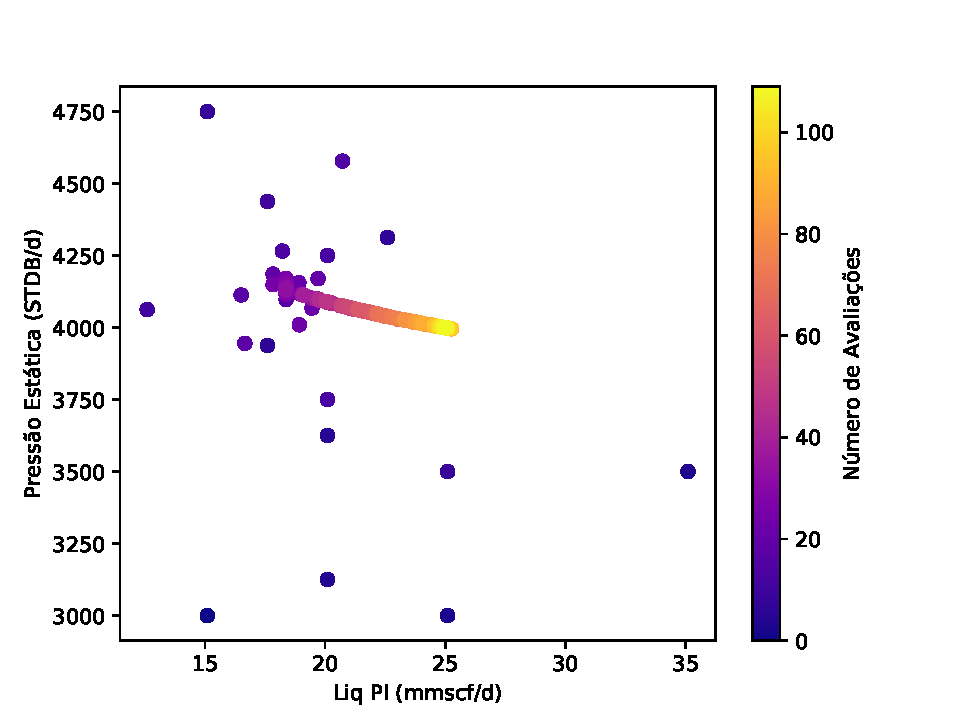
\includegraphics[width=1\linewidth]{figs/setup1nm_eval_points.pdf}
  \caption{Pontos escolhidos pelo Nelder-Mead.}
  \label{fig:setup3_points}
\end{subfigure}%
\begin{subfigure}{0.5\textwidth}
  \centering
  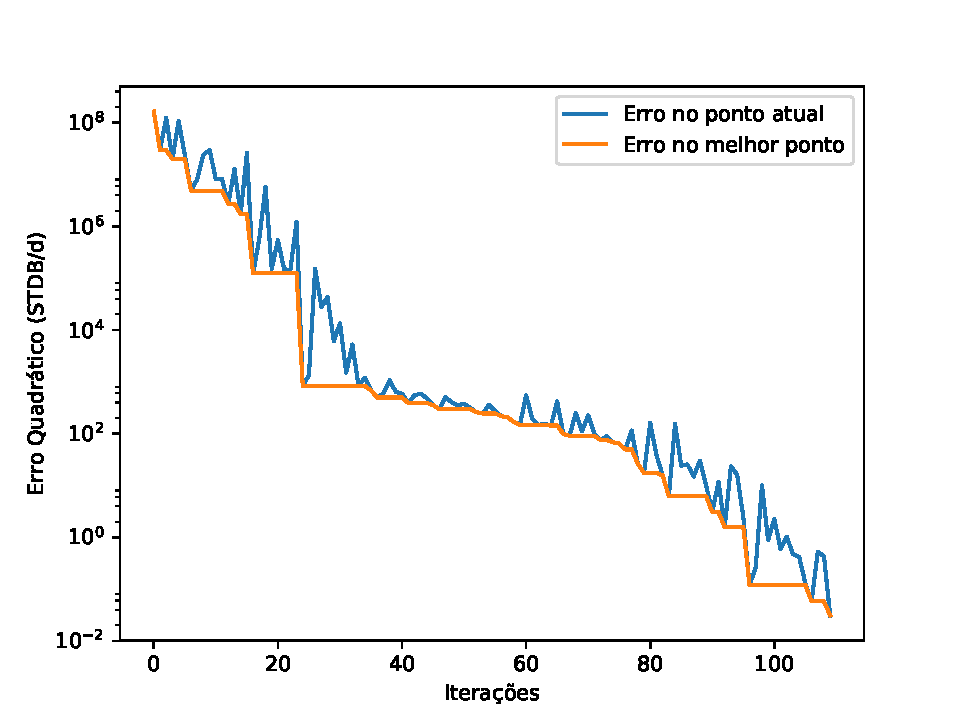
\includegraphics[width=1\linewidth]{figs/setup1nm_errors.pdf}
  \caption{Erro nos pontos avaliados.}
  \label{fig:setup3_error}
\end{subfigure}
\caption{Nelder-Mead aplicado ao experimento 1.}
\label{fig:setup3_2}
\end{figure}

\begin{figure}
\centering
	  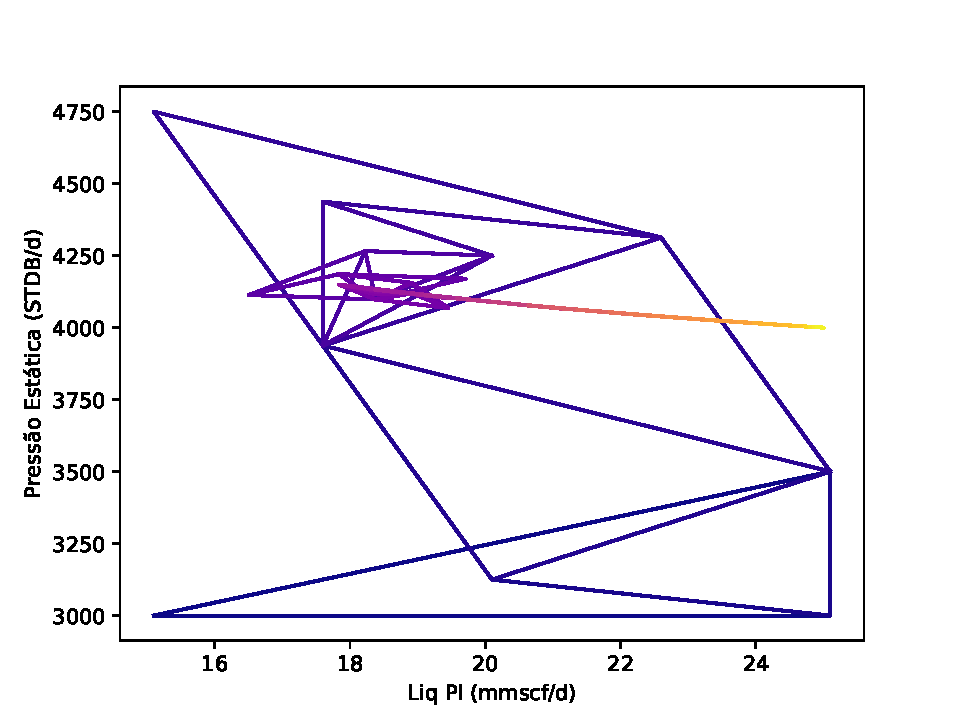
\includegraphics[width=0.7\linewidth]{figs/triangles_neldermead.pdf}
  \caption{Simplexes utilizados pelo Nelder-Mead.}
  \label{fig:setup3_triang}
\end{figure}




\section{Discussão}

É possível notar, pela figura \ref{fig:comp1} e pela \ref{tab:res1} que o Nelder-Mead, embora tenha utilizado um número semelhante de iterações que o orthoMADS, foi aproximadamente quatro vezes mais rápido. É possível que isso se dê pelo fato de que o OPAL, embora utilize várias \textit{threads}, talvez não faça um gerenciamento ideal do processador, e sim faça um \textit{busy wait}, que é quando um processo espera um sinal (no caso o fim de uma \textit{thread}) sem liberar o processador para outras \textit{threads}. Embora exista a suspeita do problema, não foi possível localizá-lo no código fonte.

Outra possível interpretação é que a diferença seja devido ao \textit{overhead} no NOMAD. Todas suas iterações envolvem o disparo de novos processos do Python, que por sua vez disparam o processo do Pipesim, além da escrita e leitura de diferentes arquivos para a comunicação entre os processos. Como a implementação utilizada do Nelder-Mead foi feita diretamente em Python, o \textit{overhead} existente é apenas a interface com Open Link.


\begin{table}[		]
\centering
\caption{Tempo de execução e numero de iterações por algoritmo}
\label{tab:res1}
\begin{tabular}{|l|l|l|}
\hline
                    & Tempo & Iterações \\ \hline
OrthoMADS           & 525   & 206       \\ \hline
OrthoMADS + SGTELIB & 1374  & 417       \\ \hline
Nelder-Mead         & 133   & 110        \\ \hline
\end{tabular}
\end{table}


\begin{figure}
\centering
  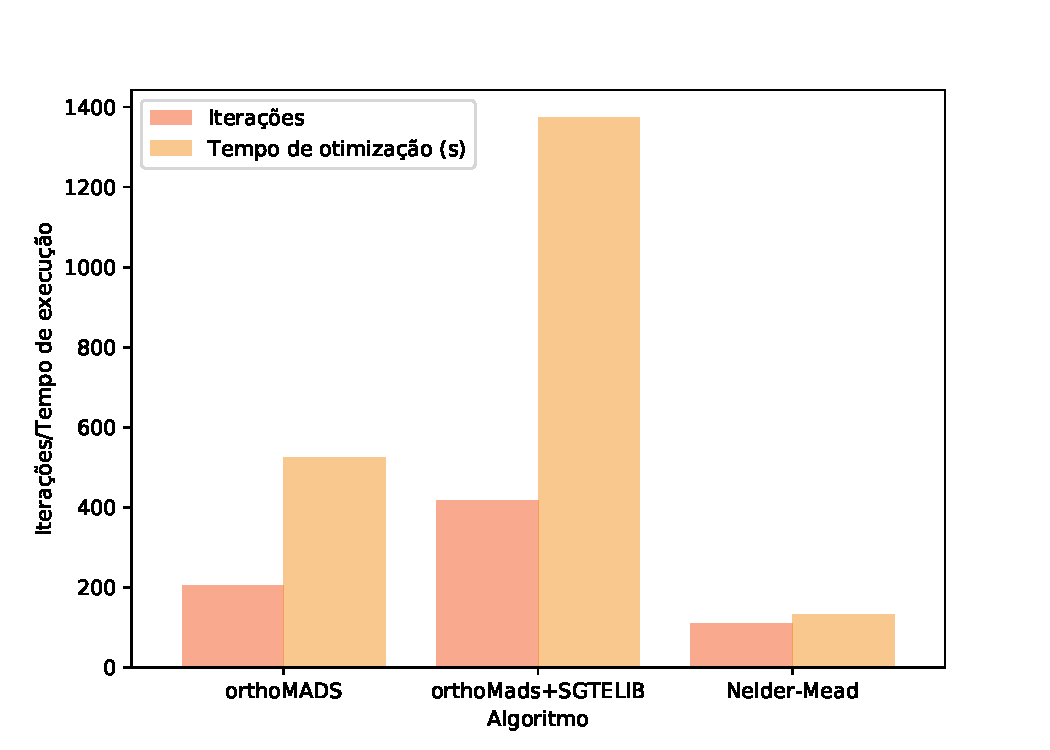
\includegraphics[width=0.7\linewidth]{figs/comp_time_iter.pdf}
  \caption{Comparação entre tempos de execução e número de iterações entre os três experimentos.}
  \label{fig:comp1}
\end{figure}


\chapter{O Experimento de Sintonia Com Ruído}

Para testar um caso um pouco mais realista, foram introduzidos ruídos ao sistema.
%
Primeiramente foi introduzido um ruído de medição nos pontos ``reais'' com desvio padrão $\sigma = 10$ (STDB/d) e média nula, para uma distribuição gaussiana.
%
Este ruído simula as condições adversas da medição em campo, perdas em sensores, sinais elétricos, imprecisões de montagem, e etc...
%
%

Adicionalmente, foi adicionado um pequeno ruído na simulação, para emular erros de precisão no caso de simuladores com soluções iterativas, que podem parar a simulação antes da precisão completa. 
%
A este ruído foi atribuído também uma distribuição normal com média zero, mas $\sigma = 10^{-5}$ para cada variável.
%
Como não existe mais a possibilidade um \textit{match} perfeito (zerar a função custo), é bom pensar no critério de parada. 
%
Como um balanço de precisão e execução, é escolhido o critério de que os pontos explorados estão a menos de $10^{-3}$ unidades de distância em cada variável.
%
Para as novas configurações, foram repetidos os experimentos.



\section{Sintonia de Curva com Ruído Com OrthoMADS}

Com o OrthoMADS, a otimização levou 334 segundos (5:34 minutos) e precisou de 130 avaliações. OS resultados podem ser analisados na figura \ref{fig:exp2_om}, que mostra os pontos avaliados e progressão do erro com as avaliações, e na figura \ref{fig:exp2_om_curve}, aonde é possível notar que a curva identificada está muito próxima a real, apesar do ruído na curva medida. 




\begin{figure}
\centering
\begin{subfigure}{0.5\textwidth}
  \centering
  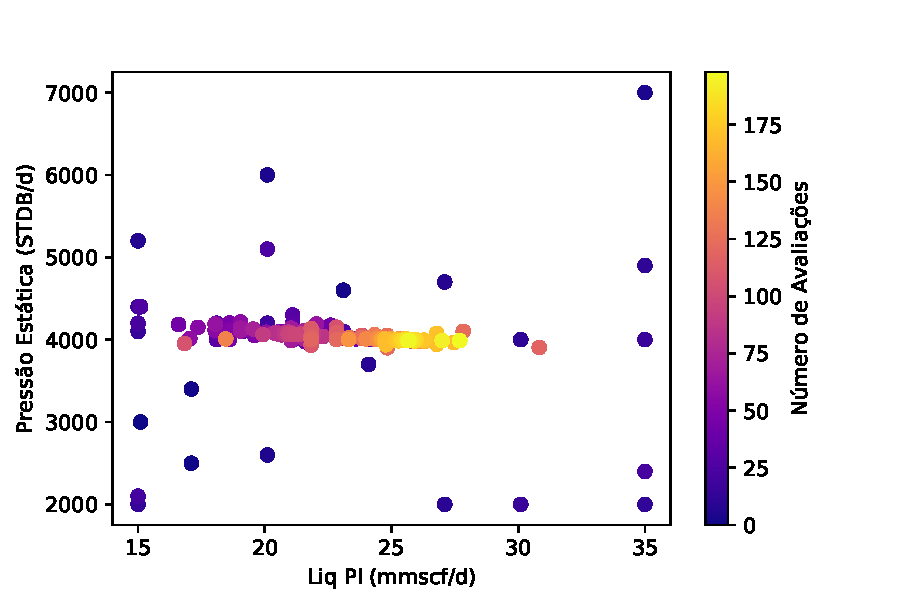
\includegraphics[width=1\linewidth]{figs/setup2_om_points.pdf}
  \caption{Pontos escolhidos pelo NOMAD.}
  \label{fig:exp2_om_points}
\end{subfigure}%
\begin{subfigure}{0.5\textwidth}
  \centering
  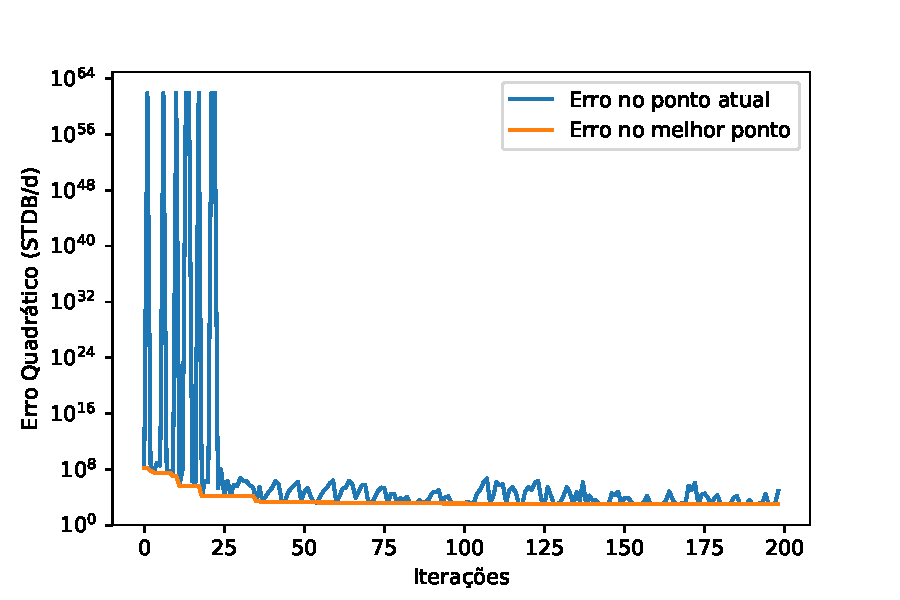
\includegraphics[width=1\linewidth]{figs/setup2_om_errors.pdf}
  \caption{Erro nos pontos avaliados.}
  \label{fig:exp2_om_error}
\end{subfigure}
\caption{NOMAD aplicado ao experimento 2.}
\label{fig:exp2_om}
\end{figure}





\begin{figure}
\centering
  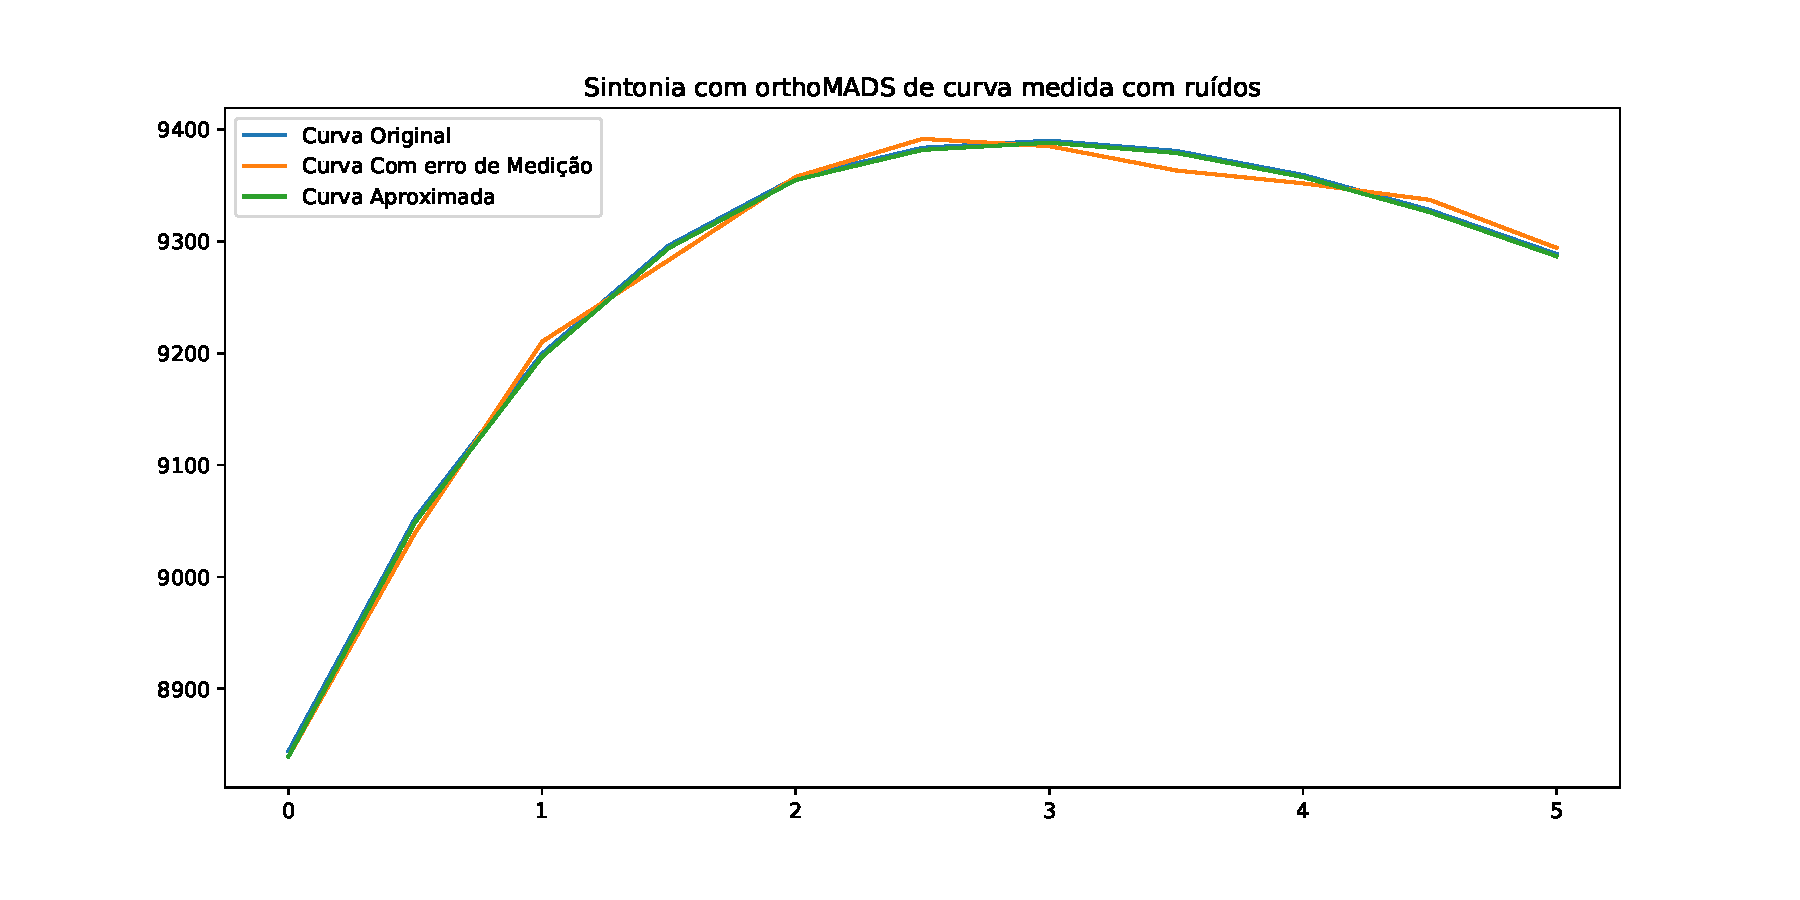
\includegraphics[width=1\linewidth]{figs/curva_om.pdf}
  \caption{Resultado da sintonia utilizando-se o OrthoMADS.}
  \label{fig:exp2_om_curve}
\end{figure}




\section{Sintonia de Curva com Ruído Com OrthoMADS + SGTELIB}

Com o OrthoMADS e a SGTELIB, a otimização levou 187 segundos (3:07 minutos) e precisou de 68 avaliações de caixa preta. Os resultados podem ser avaliados na figura \ref{fig:exp2_sg}, que mostra os pontos avaliados e progressão do erro com as avaliações, e na figura \ref{fig:exp2_sg_curve}, aonde é possível notar que a curva identificada também está muito próxima a real, apesar do ruído na curva medida. 
%

Também é notável que o novo método de SEARCH foi capaz de diminuir o número de avaliações (52\%).
%
Ele converge para um ponto próximo ao do método anterior (respectivamente 982,524 e 956,827), consumindo menos tempo e avaliações.


\begin{figure}[H]
\centering
\begin{subfigure}{0.5\textwidth}
  \centering
  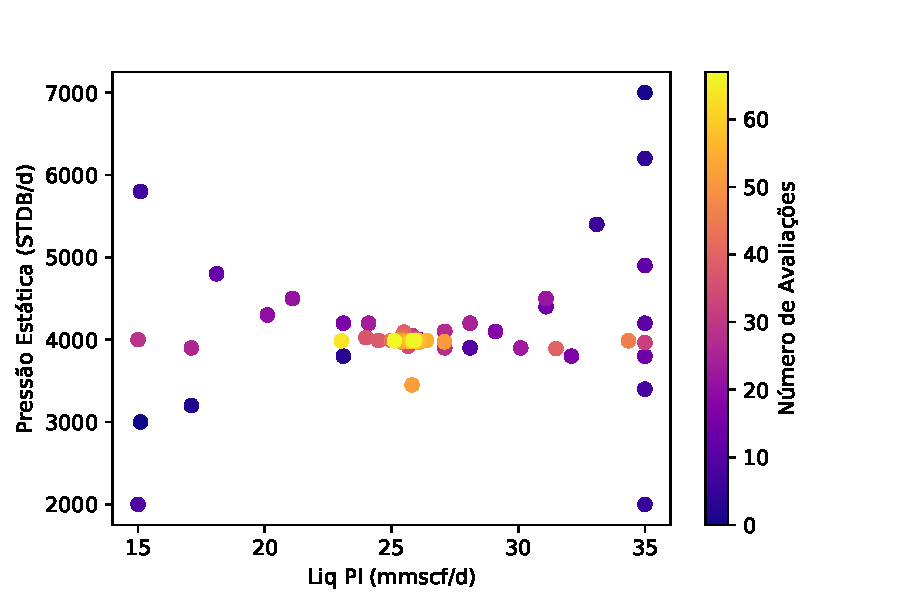
\includegraphics[width=1\linewidth]{figs/setup2_sg_points.pdf}
  \caption{Pontos escolhidos pelo NOMAD.}
  \label{fig:exp2_sg_points}
\end{subfigure}%
\begin{subfigure}{0.5\textwidth}
  \centering
  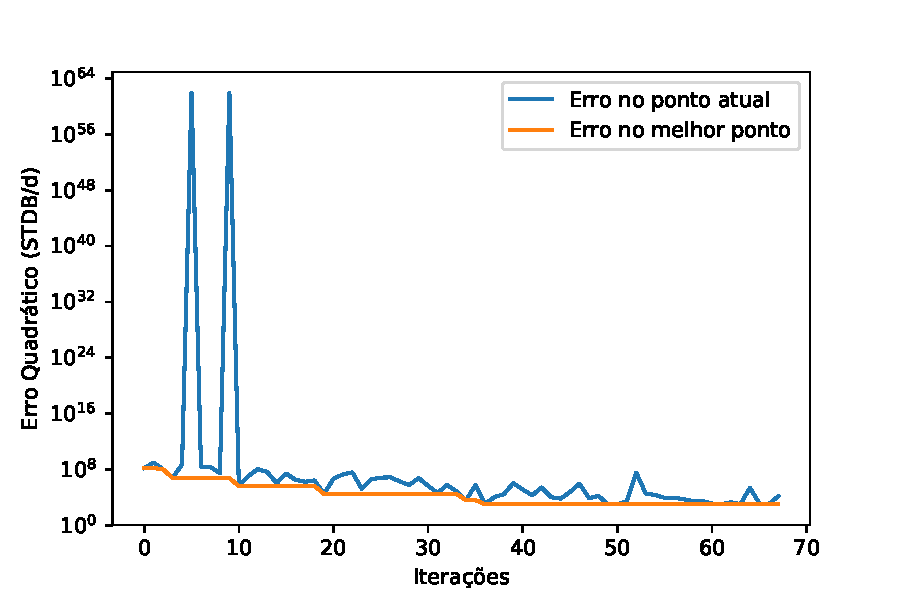
\includegraphics[width=1\linewidth]{figs/setup2noisy_sg_errors.pdf}
  \caption{Erro nos pontos avaliados.}
  \label{fig:exp2_sg_error}
\end{subfigure}
\caption{NOMAD com SGTELIB aplicado ao experimento 2.}
\label{fig:exp2_sg}
\end{figure}





\begin{figure}[H]
\centering
  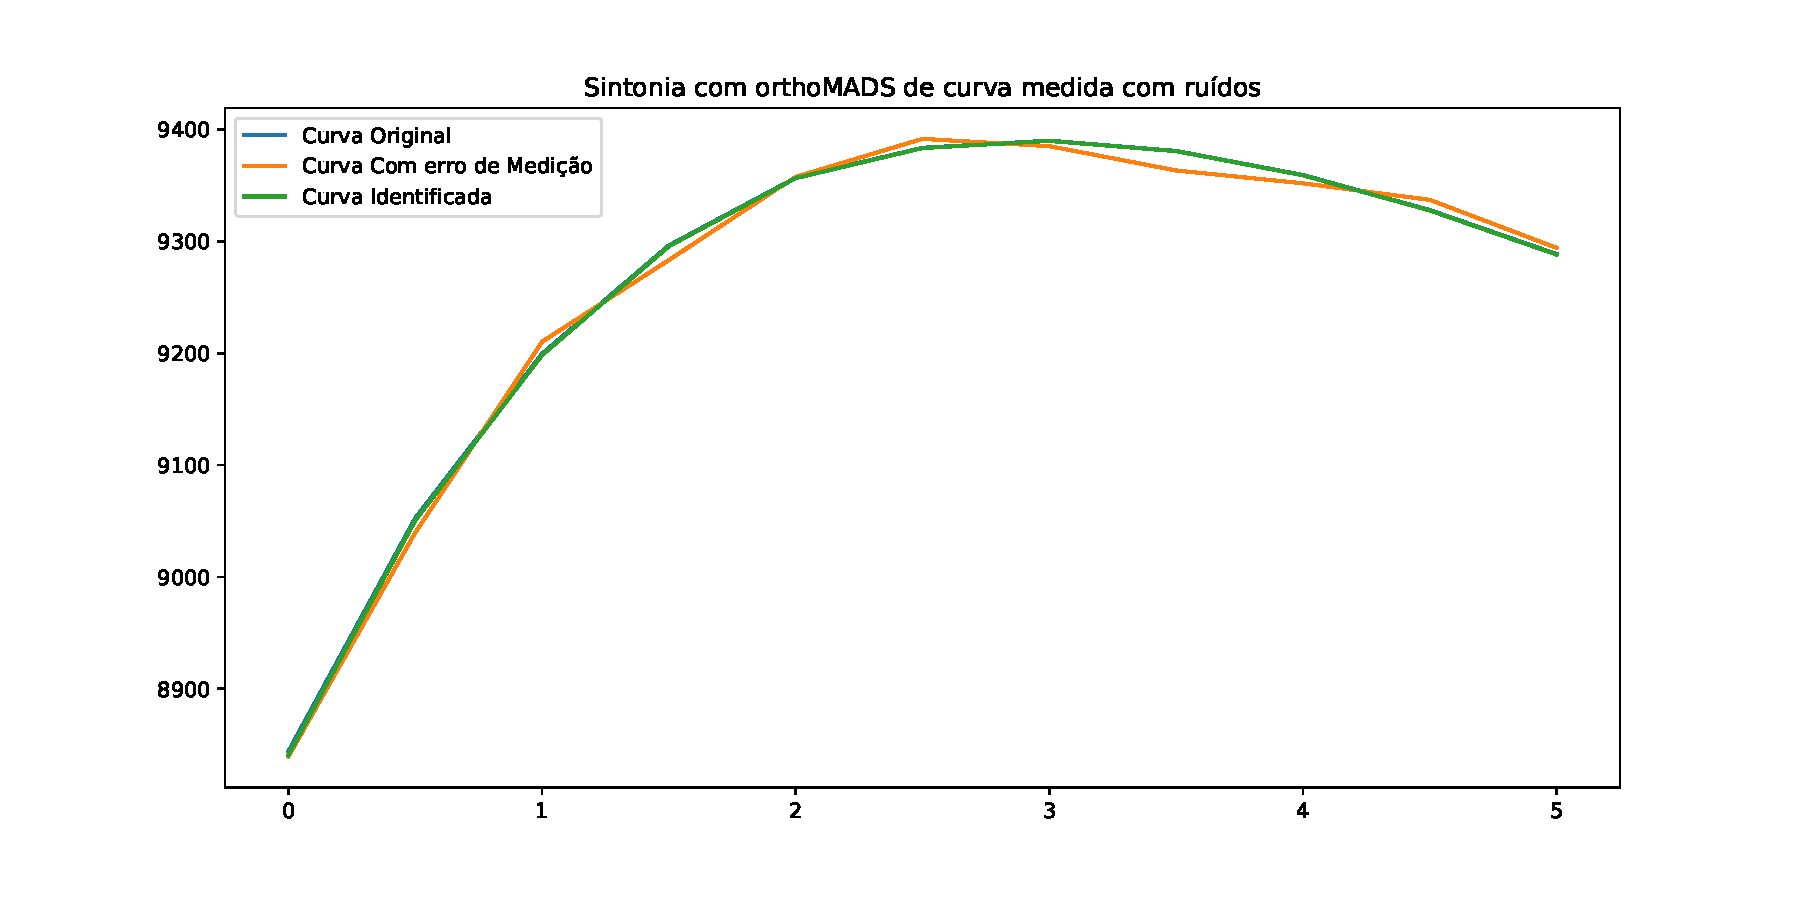
\includegraphics[width=1\linewidth]{figs/curva_sg.pdf}
  \caption{Resultado da sintonia utilizando-se o OrthoMADS com a SGTELIB.}
  \label{fig:exp2_sg_curve}
\end{figure}


\section{Sintonia de Curva com Ruído Com Nelder-Mead}

Com a utilização do algoritmo de Nelder-Mead, em 217 segundos (3:27 minutos) e 92 avaliações, o algoritmo convergiu com uma uma função custo em 953.623. Como pode se ver na figura \ref{fig:exp2_nm_error}, o algoritmo converge rapidamente no inicial, mas demora a adquirir a precisão requerida para a parada. Novamente a curva identificada está muito próxima da original sem ruídos.



\begin{figure}[H]
\centering
\begin{subfigure}{0.5\textwidth}
  \centering
  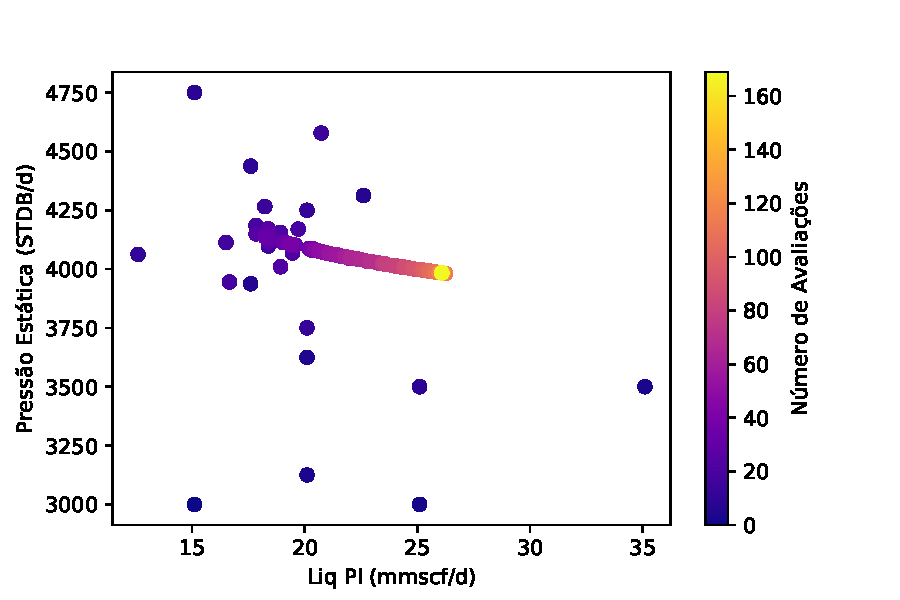
\includegraphics[width=1\linewidth]{figs/setup2_nm_points.pdf}
  \caption{Pontos testados pelo Nelder-Mead.}
  \label{fig:exp2_nm_points}
\end{subfigure}%
\begin{subfigure}{0.5\textwidth}
  \centering
  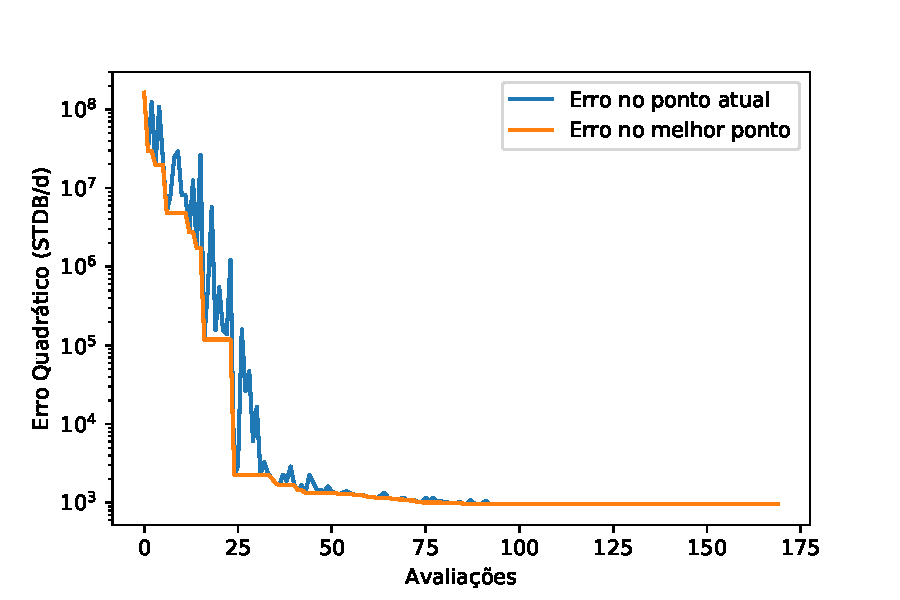
\includegraphics[width=1\linewidth]{figs/setup2_nm_errors.pdf}
  \caption{Erro nos pontos avaliados.}
  \label{fig:exp2_nm_error}
\end{subfigure}
\caption{Nelder-Mead aplicado ao experimento 2.}
\label{fig:exp2_nm}
\end{figure}





\begin{figure}[H]
\centering
  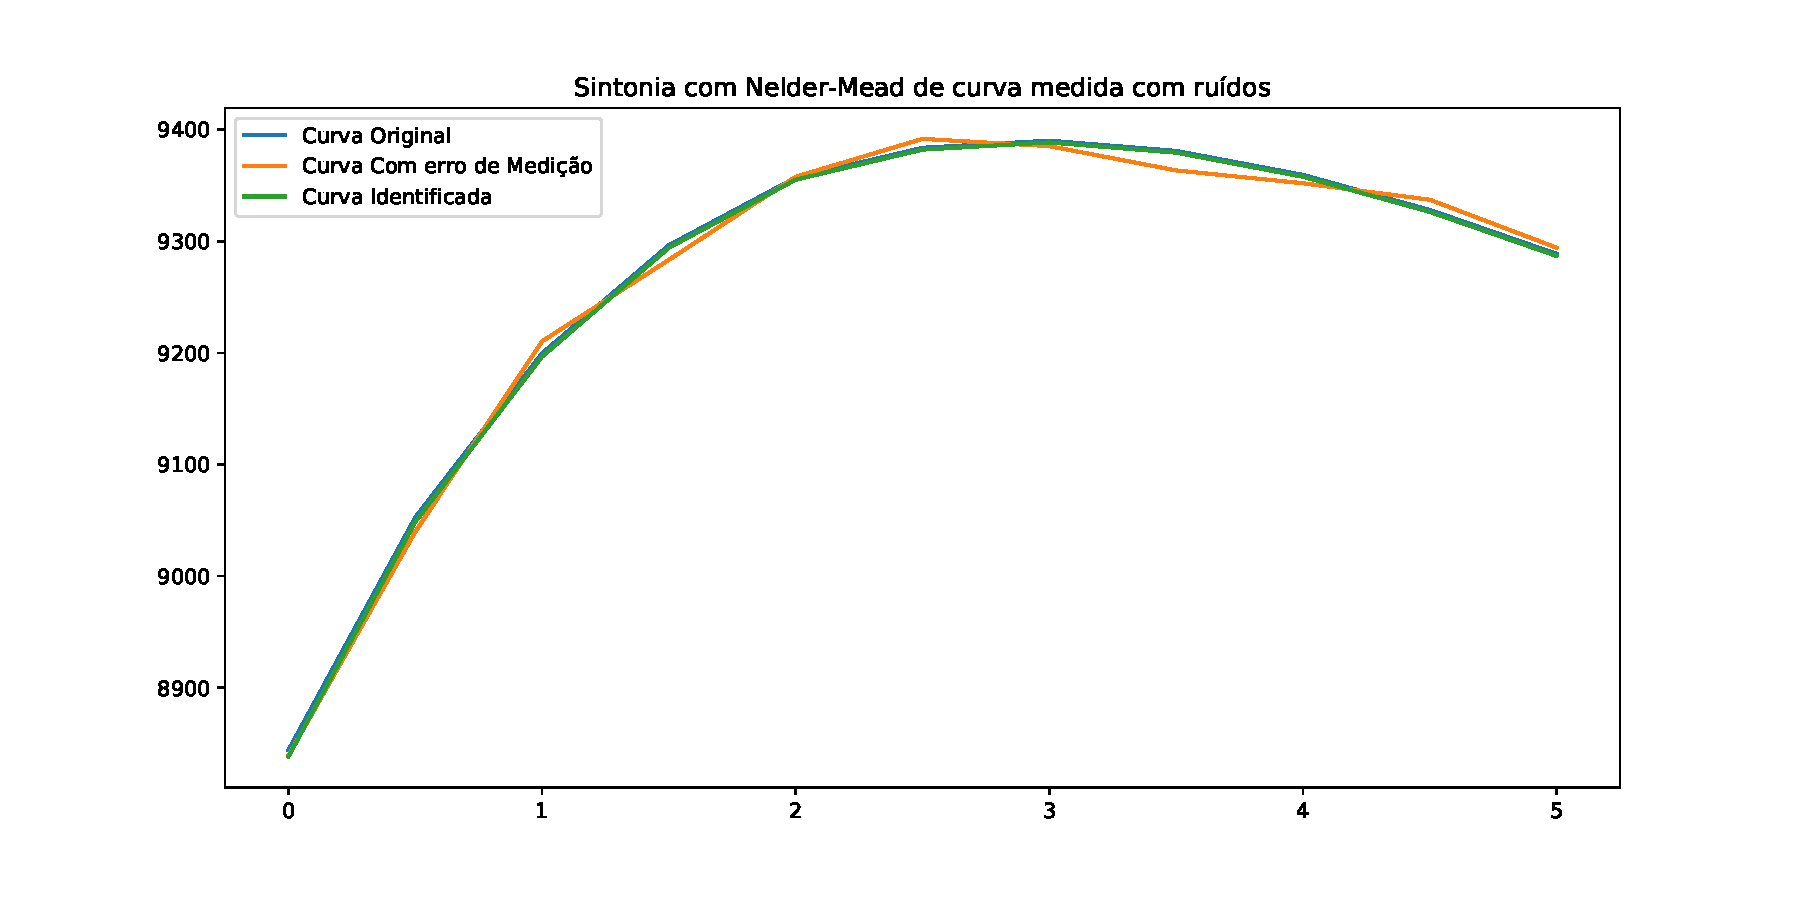
\includegraphics[width=1\linewidth]{figs/curva_nm.pdf}
  \caption{Resultado da sintonia utilizando-se o Nelder-Mead.}
  \label{fig:exp2_nm_curve}
\end{figure}

\section{Discussão}
Nestes experimentos com ruído, não se repete o comportamento anômalo aonde o Nomad com SGTELIB avalia pontos em que aparentemente não há informações relevantes, aumentando sem necessidade o número de iterações e tempo computacional, como pode ser visto na Figura \ref{fig:comp2} e na Tabela \ref{tab:res2}.
%
Pelo contrário, ele acaba sendo o mais eficiente dos três métodos. O Nelder-Mead, por sua vez, tornou-se relativamente mais lento.

%

%

\begin{table}[H]
\centering
\caption{Comparação dos métodos para sintonia de uma curva com ruído de medição}
\label{tab:res2}
\begin{tabular}{|l|l|l|l|}
\hline
                    & Tempo & Iterações & Custo   \\ \hline
OrthoMADS           & 334   & 130       & 956,827 \\ \hline
OrthoMADS + SGTELIB & 187   & 68        & 982,524 \\ \hline
Nelder-Mead         & 217   & 92        & 953,522 \\ \hline
\end{tabular}
\end{table}




\begin{figure}[H]
\centering
  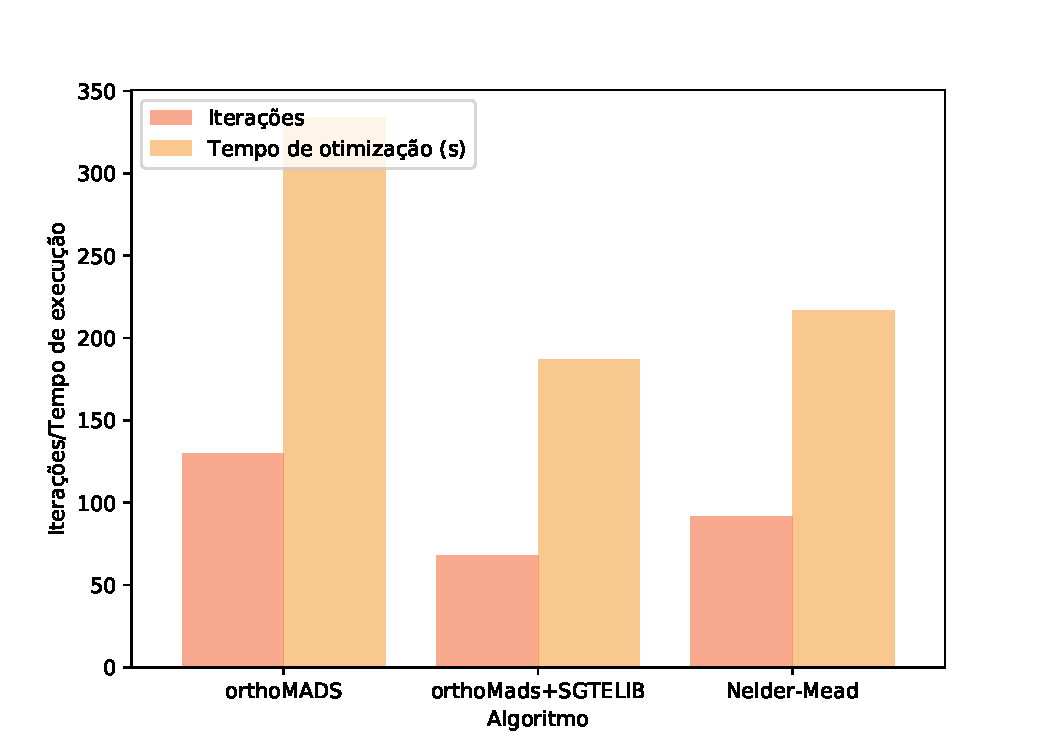
\includegraphics[width=0.7\linewidth]{figs/comp_time_iter_2.pdf}
  \caption{Comparação entre tempos de execução e número de iterações entre os três experimentos com ruído.}
  \label{fig:comp2}
\end{figure}






%%%%%%%%%%%%%%%%%%%